\documentclass[11pt]{article}
\usepackage[utf8]{inputenc}
\usepackage[T1]{fontenc}
\usepackage{amsmath, amssymb, amsthm, mathtools}
\usepackage{mathrsfs}
\usepackage{enumitem}
\usepackage{booktabs}
\usepackage{array}
\usepackage{hyperref}
\hypersetup{
    colorlinks=true,
    linkcolor=blue,
    citecolor=blue,
    urlcolor=blue
}
\usepackage{tikz}
\usetikzlibrary{positioning}

\newtheorem{theorem}{Theorem}[section]
\newtheorem{lemma}[theorem]{Lemma}
\newtheorem{proposition}[theorem]{Proposition}
\newtheorem{corollary}[theorem]{Corollary}
\newtheorem{definition}[theorem]{Definition}
\newtheorem{remark}[theorem]{Remark}
\newtheorem{example}[theorem]{Example}
\newtheorem{conjecture}[theorem]{Conjecture}

\newcommand{\N}{\mathbb{N}}
\newcommand{\Z}{\mathbb{Z}}
\newcommand{\R}{\mathbb{R}}
\newcommand{\cT}{\mathcal{T}}
\newcommand{\cB}{\mathcal{B}}
\newcommand{\skel}{\mathrm{skel}}
\newcommand{\Aut}{\mathrm{Aut}}
\newcommand{\sep}{\mathrm{sep}}
\newcommand{\ord}{\mathrm{ord}}
\newcommand{\conn}{\mathrm{conn}}
\newcommand{\BC}{\mathrm{BC}}
\newcommand{\sepset}{\mathcal{S}}

\title{Canonical Tree Decompositions of Graphs: \\ From Blocks to $k$-Blocks and Beyond}
\author{Anonymous Author}
\date{}

\begin{document}

\maketitle

\begin{abstract}
    We present a unified framework for canonical tree decompositions of finite graphs based on vertex separators of increasing size. Starting from the classical block--cut tree (decomposing along 1-separators), we systematically develop the SPQR-tree (2-separators), the quasi-4-connected decomposition (3-separators), and the general $(k+1)$-block decomposition hierarchy. A central theme is the distinction between \emph{local connectivity} (induced subgraphs) and \emph{global inseparability} (paths possibly leaving the vertex set). We prove that $k$-blocks---maximal vertex sets pairwise $(k\!-\!1)$-inseparable in the whole graph---need not induce $k$-connected subgraphs, resolving a subtle misconception in the literature. For $k \geq 3$, crossing $k$-separators obstruct decomposition into strictly $(k+1)$-connected components; we show how \emph{quasi-$(k+1)$-connectivity} overcomes this via tangle theory. The paper culminates in a precise definition of the canonical $(k+1)$-block decomposition tree that displays all maximal $(k+1)$-blocks within a $k$-block, establishing existence, uniqueness, and algorithmic properties for all $k \geq 1$.
\end{abstract}

\section{Introduction}
\label{sec:intro}

Structural graph theory seeks to decompose complex graphs into simpler, highly connected pieces arranged in a tree-like hierarchy. The most celebrated examples are:
\begin{itemize}[leftmargin=*,nosep]
    \item The \emph{block--cut tree}, decomposing graphs along cut vertices (1-separators) into 2-connected blocks,
    \item The \emph{SPQR-tree}, decomposing biconnected graphs along separation pairs (2-separators) into triconnected components.
\end{itemize}
These decompositions are \emph{canonical} (invariant under automorphisms), computable in linear time, and fundamental to graph drawing, planarity testing, and network reliability.

A natural question arises: \emph{Can we continue this hierarchy to decompose triconnected graphs along 3-separators into 4-connected pieces, and so on?} The answer is subtle. While SPQR-trees decompose graphs into \emph{triconnected components} (R-nodes), these do not coincide with \emph{3-blocks} in the modern sense of Carmesin et al.~\cite{carmesin2014canonical}. Moreover, for $k \geq 3$, $k$-separators may \emph{cross}, preventing decomposition into strictly $(k+1)$-connected components.

This paper synthesizes three decades of research into a coherent framework:
\begin{enumerate}
    \item We clarify the precise relationship between classical decompositions (block--cut, SPQR) and the modern theory of $k$-blocks.
    \item We prove that the vertex set of a $k$-block need not induce a $k$-connected subgraph---a critical distinction between \emph{global inseparability} and \emph{local connectivity}.
    \item We define \emph{quasi-$(k+1)$-connectivity} to handle crossing separators, yielding canonical decompositions for all $k$.
    \item We present the complete hierarchy of canonical tree decompositions displaying $(k+1)$-blocks within $k$-blocks.
\end{enumerate}

Our main contribution is Definition~\ref{def:kplus1-decomp}, which formalizes the $(k+1)$-block decomposition tree for arbitrary $k \geq 1$, together with Theorem~\ref{thm:existence} establishing its existence and uniqueness. We include explicit counterexamples demonstrating why ``quasi'' connectivity is unavoidable for $k \geq 3$, and why R-nodes do not represent 3-blocks.

\section{Preliminaries}
\label{sec:prelim}

All graphs are finite, simple (unless otherwise noted for SPQR skeletons), and undirected. For a graph $G = (V,E)$ and $S \subseteq V$, denote by $G - S$ the graph obtained by deleting vertices in $S$ and their incident edges.

\begin{definition}[Separator and separation]
    A vertex set $S \subseteq V$ is a \emph{$k$-separator} if $|S| = k$ and $G - S$ has at least two connected components. A \emph{separation} of $G$ is an ordered pair $(A,B)$ of vertex sets such that $A \cup B = V$ and there is no edge between $A \setminus B$ and $B \setminus A$. The \emph{order} of $(A,B)$ is $|A \cap B|$.
\end{definition}

\begin{definition}[$k$-inseparability and $k$-blocks]
    Two vertices $u,v \in V$ are \emph{$(k-1)$-inseparable} if no set $S \subseteq V \setminus \{u,v\}$ with $|S| < k$ separates $u$ from $v$ in $G$. A \emph{$k$-block} is a maximal vertex set $B \subseteq V$ with $|B| \geq k$ such that every pair of vertices in $B$ is $(k-1)$-inseparable.
\end{definition}

Note that $k$-blocks are defined by a \emph{global} property: paths connecting vertices of $B$ may leave $B$ and traverse vertices outside $B$. This contrasts with the \emph{local} property of the induced subgraph $G[B]$ being $k$-connected.

\begin{definition}[Crossing separators]
    Two $k$-separators $S_1, S_2$ \emph{cross} if at least two components of $G - S_1$ each contain vertices of $V \setminus S_2$, and vice versa. Otherwise, they are \emph{nested}.
\end{definition}

Crossing separators are the fundamental obstruction to tree-like decompositions for $k \geq 3$ (see Section~\ref{sec:quasi}).

\section{Block--Cut Tree Decomposition ($k=1$)}
\label{sec:blockcut}

The block--cut tree decomposes a connected graph along cut vertices (1-separators).

\begin{definition}[Block]
    A \emph{block} of $G$ is a maximal connected subgraph containing no cut vertex. Equivalently, a block is either:
    \begin{enumerate}[label=(\roman*)]
        \item a maximal 2-connected subgraph ($|V| \geq 3$),
        \item a bridge (an edge whose removal disconnects $G$, isomorphic to $K_2$), or
        \item an isolated vertex ($K_1$, occurring only when $|V| = 1$).
    \end{enumerate}
\end{definition}

\begin{definition}[Block--cut tree]
    The \emph{block--cut tree} of a connected graph $G$, denoted $\BC(G)$, is a bipartite tree $\cT = (W_B \cup W_C, F)$ where:
    \begin{itemize}
        \item $W_B$ contains one node for each block of $G$,
        \item $W_C$ contains one node for each cut vertex of $G$,
        \item $bc \in F$ iff the cut vertex represented by $c$ belongs to the block represented by $b$.
    \end{itemize}
\end{definition}

The block--cut tree is canonical, unique, and computable in linear time. Its bags (corresponding to blocks) induce 2-connected subgraphs \emph{except} for bridges and isolated vertices. Crucially, the vertex set of a 2-block (maximal 2-inseparable set) \emph{does} induce a 2-connected subgraph---a special property that fails for $k \geq 3$.

\section{SPQR-Tree Decomposition ($k=2$)}
\label{sec:spqr}

The SPQR-tree decomposes a biconnected graph along separation pairs (2-separators).

\begin{definition}[Separation pair]
    A \emph{separation pair} of a biconnected graph $G$ is a 2-separator $\{u,v\}$ such that $G - \{u,v\}$ is disconnected.
\end{definition}

\begin{definition}[SPQR-tree]
    Let $G$ be biconnected with $|V| \geq 3$. An \emph{SPQR-tree} of $G$ is a tree $\cT = (W,F)$ together with a skeleton assignment $\skel : W \to \{\text{multigraphs}\}$ satisfying:
    \begin{enumerate}[label=(\roman*)]
        \item Each node $\mu \in W$ has one of four types:
        \begin{description}
            \item[S-node (Series):] $\skel(\mu)$ is a simple cycle of length $\geq 3$.
            \item[P-node (Parallel):] $\skel(\mu)$ consists of two vertices joined by $\geq 3$ parallel edges.
            \item[R-node (Rigid):] $\skel(\mu)$ is a 3-connected simple graph with $\geq 4$ vertices.
            \item[Q-node (Edge):] $\skel(\mu)$ is a single real edge of $G$ (often omitted).
        \end{description}
        
        \item Each tree edge $e = \mu\nu$ corresponds to a \emph{virtual edge} $\varepsilon_e$ appearing in both $\skel(\mu)$ and $\skel(\nu)$.
        
        \item $G$ is reconstructible by iteratively merging adjacent skeletons along virtual edges via 2-sums.
    \end{enumerate}
\end{definition}

The SPQR-tree is canonical and computable in linear time~\cite{hopcroft1973dividing, battista1996online}. Its R-nodes represent \emph{triconnected components}---maximal 3-connected subgraphs up to 2-sums. However, as we now show, R-nodes do \emph{not} represent 3-blocks in the Carmesin sense.

\section{3-Blocks vs.\ R-Nodes: A Critical Distinction}
\label{sec:3blocks}

A common misconception is that R-nodes represent 3-blocks. This is false: 3-blocks are defined by global inseparability, while R-nodes capture local triconnectivity after decomposition.

\begin{theorem}
    \label{thm:3block-not-3conn}
    The induced subgraph on the vertex set of a 3-block need not be 3-connected. Similarly, the vertex set corresponding to an R-node need not induce a 3-connected subgraph in $G$.
\end{theorem}

\begin{proof}
    Consider the graph $G$ with vertex set $V = \{v_1,v_2,v_3,v_4,x,y\}$ and edge set
    \[
        E = \{v_1v_2, v_2v_3, v_3v_4, v_4v_1, xv_1, xv_3, yv_2, yv_4\}.
    \]
    (No edge between $x$ and $y$; see Figure~\ref{fig:counterexample}.)
    
    Let $B = \{v_1,v_2,v_3,v_4\}$. We claim $B$ is a maximal 3-block:
    \begin{itemize}
        \item \emph{3-inseparability}: For any $u,v \in B$ and any 2-set $S \subseteq V \setminus \{u,v\}$, $u$ and $v$ remain connected in $G - S$. For example:
        \begin{itemize}
            \item Pair $(v_1,v_3)$ with $S = \{v_2,v_4\}$: path $v_1$--$x$--$v_3$ survives.
            \item Pair $(v_2,v_4)$ with $S = \{v_1,v_3\}$: path $v_2$--$y$--$v_4$ survives.
            \item Pair $(v_1,v_2)$ with $S = \{v_3,v_4\}$: direct edge $v_1v_2$ survives.
        \end{itemize}
        \item \emph{Maximality}: Adding $x$ fails---pair $(x,v_2)$ is separated by $S = \{v_1,v_3\}$ (removing $v_1,v_3$ isolates $x$ while $v_2$ connects to $y$). Similarly for $y$.
    \end{itemize}
    However, $G[B]$ is the 4-cycle $v_1v_2v_3v_4v_1$, which has vertex connectivity 2. The set $\{v_1,v_3\}$ is a 2-separator in $G[B]$ (disconnecting $v_2$ from $v_4$), though globally in $G$ the pair remains connected via $y$.
    
    Thus $B$ is a 3-block whose induced subgraph is not 3-connected.
\end{proof}

\begin{figure}[h]
    \centering
    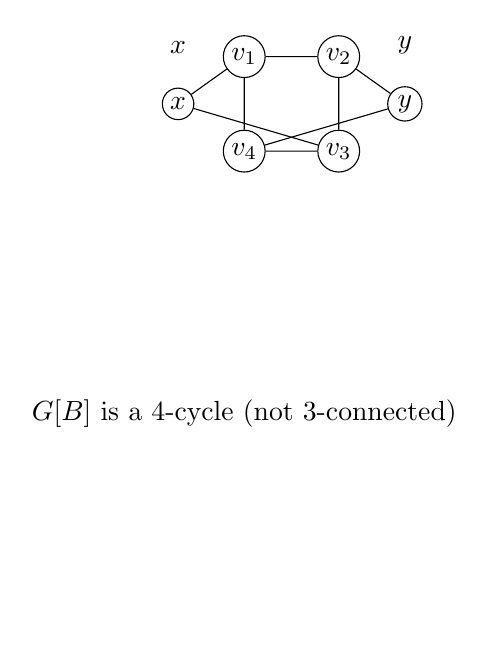
\begin{tikzpicture}[scale=1.2, every node/.style={circle, draw, inner sep=1.5pt}]
        \node (v1) at (0,1) {$v_1$};
        \node (v2) at (1,1) {$v_2$};
        \node (v3) at (1,0) {$v_3$};
        \node (v4) at (0,0) {$v_4$};
        \node (x) at (-0.7,0.5) {$x$};
        \node (y) at (1.7,0.5) {$y$};
        
        \draw (v1) -- (v2) -- (v3) -- (v4) -- (v1);
        \draw (x) -- (v1);
        \draw (x) -- (v3);
        \draw (y) -- (v2);
        \draw (y) -- (v4);
        
        \node[draw=none, below=0.3cm of v4] {$G[B]$ is a 4-cycle (not 3-connected)};
        \node[draw=none, above=0.3cm of x] {$x$};
        \node[draw=none, above=0.3cm of y] {$y$};
    \end{tikzpicture}
    \caption{Counterexample: $B = \{v_1,v_2,v_3,v_4\}$ is a 3-block, but $G[B]$ has connectivity 2.}
    \label{fig:counterexample}
\end{figure}

\begin{remark}
    \begin{enumerate}[label=(\roman*)]
        \item The SPQR-tree of $G$ contains a single R-node whose skeleton is $K_4$ (with virtual edges replacing paths through $x$ and $y$). Yet the R-node's vertex set $\{v_1,v_2,v_3,v_4\}$ induces a subgraph of connectivity 2.
        
        \item This phenomenon occurs whenever a 2-separator is ``healed'' globally by vertices outside the set. The 3-block captures global cohesion; the induced subgraph reflects only local structure.
        
        \item For $k=2$, 2-blocks \emph{do} induce 2-connected subgraphs. The failure begins at $k=3$ due to the possibility of crossing separators (absent for $k=1,2$).
    \end{enumerate}
\end{remark}

\section{Quasi-4-Connectivity and 4-Block Decomposition ($k=3$)}
\label{sec:quasi}

For $k \geq 3$, $k$-separators may cross, preventing decomposition into strictly $(k+1)$-connected components. Grohe~\cite{grohe2016quasi} resolved this for $k=3$ using \emph{quasi-4-connectivity}.

\begin{definition}[Quasi-4-connected graph]
    A 3-connected graph $H$ is \emph{quasi-4-connected} if for every 3-separator $S$ of $H$, at most one component of $H - S$ contains more than one vertex, and all 3-separators of $H$ are nested.
\end{definition}

Quasi-4-connected graphs may contain 3-separators, but these are ``inessential'': they do not split the graph into multiple large pieces, and they do not cross.

\begin{theorem}[Grohe 2016]
    Every triconnected graph $G$ admits a canonical tree decomposition $\cT_4(G)$ of adhesion 3 whose torsos are quasi-4-connected. This decomposition displays all maximal 4-blocks of $G$.
\end{theorem}

The decomposition is unique up to isomorphism and computable in $O(|V|^2)$ time. Crucially:
\begin{itemize}
    \item A single 4-block may span multiple adjacent bags if connected by inessential 3-separators.
    \item Quasi-4-connected torsos need not be 4-connected (e.g., a wheel graph $W_5$ with a subdivided spoke).
\end{itemize}

\section{General $(k+1)$-Block Decomposition Hierarchy}
\label{sec:general}

We now present the complete hierarchy unifying all previous levels.

\begin{definition}[Essential $k$-separator for a $k$-block]
    Let $B$ be a $k$-block of $G$. A $k$-separator $S$ is \emph{essential for $B$} if there exist $u,v \in B \setminus S$ such that every $u$-$v$ path in $G$ intersects $S$. Otherwise, $S$ is \emph{inessential}.
\end{definition}

\begin{definition}[Quasi-$(k+1)$-connected component]
    \label{def:quasi}
    A subgraph $H \subseteq G$ is \emph{quasi-$(k+1)$-connected} if:
    \begin{enumerate}[label=(\roman*)]
        \item $H$ is $k$-connected,
        \item Every $k$-separator of $H$ is inessential for $V(H)$ within $G$,
        \item All $k$-separators of $H$ are nested.
    \end{enumerate}
\end{definition}

\begin{definition}[$(k+1)$-block decomposition tree]
    \label{def:kplus1-decomp}
    Let $B$ be a $k$-block of $G$ with $k \geq 1$. A \emph{$(k+1)$-block decomposition} of $B$ is a tree $\cT_{k+1}(B) = (W,F)$ together with:
    \begin{itemize}
        \item A family of vertex sets $\{X_\mu \subseteq B \mid \mu \in W\}$ (bags),
        \item For each edge $e = \mu\nu \in F$, a separator label $S_e \subseteq B$ with $|S_e| = k$,
    \end{itemize}
    satisfying:
    \begin{enumerate}[label=(\roman*)]
        \item \textbf{Adhesion:} $X_\mu \cap X_\nu = S_{\mu\nu}$ for all $\mu\nu \in F$.
        
        \item \textbf{Essential separator coverage:} Every essential $k$-separator for $B$ equals $S_e$ for some $e \in F$.
        
        \item \textbf{Quasi-connectivity:} For each $\mu \in W$, $G[X_\mu]$ is quasi-$(k+1)$-connected.
        
        \item \textbf{$(k+1)$-block display:} Each maximal $(k+1)$-block $B' \subseteq B$ is contained in a unique bag $X_\mu$ with $|X_\mu| < |B'| + k + 1$, and for every neighbor $\nu$ of $\mu$, $S_{\mu\nu}$ does not separate any two vertices of $B'$.
        
        \item \textbf{Canonicity:} $\cT_{k+1}(B)$ is invariant under $\Aut(G)_B = \{\phi \in \Aut(G) \mid \phi(B) = B\}$.
    \end{enumerate}
\end{definition}

\begin{theorem}[Existence and uniqueness]
    \label{thm:existence}
    For every $k \geq 1$ and every $k$-block $B$ of a finite graph $G$, there exists a canonical $(k+1)$-block decomposition tree $\cT_{k+1}(B)$ satisfying Definition~\ref{def:kplus1-decomp}. It is unique up to tree isomorphism preserving separator labels.
\end{theorem}

\begin{proof}[Sketch]
    The decomposition arises from the canonical tree decomposition of the tangle of order $k+1$ corresponding to the $k$-block $B$ (Robertson--Seymour~\cite{robertson1991graph}, Carmesin et al.~\cite{carmesin2014canonical}). Tangles provide a unified framework where crossing separators are absorbed into bounded-size ``junctions,'' yielding quasi-$(k+1)$-connected torsos. Canonicity follows from the tangle's invariance under automorphisms stabilizing $B$.
\end{proof}

\begin{table}[h]
    \centering
    \caption{Hierarchy of canonical tree decompositions}
    \label{tab:hierarchy}
    \begin{tabular}{c c c c c c}
        \toprule
        Level & Separator size & Decomposition & Component type & Crossing separators? & Strict $(k+1)$-connectivity? \\
        \midrule
        $k=1$ & 1 & Block--cut tree & 2-blocks & Impossible & Yes \\
        $k=2$ & 2 & SPQR-tree & Triconnected components & Impossible & Yes \\
        $k=3$ & 3 & 4-block tree & Quasi-4-connected & Possible & No (quasi only) \\
        $k \geq 4$ & $k$ & $(k+1)$-block tree & Quasi-$(k+1)$-connected & Ubiquitous & No (quasi only) \\
        \bottomrule
    \end{tabular}
\end{table}

\section{Tangles: The Unifying Framework}
\label{sec:tangles}

The deepest explanation for this hierarchy comes from tangle theory~\cite{robertson1991graph}.

\begin{definition}[Tangle]
    A \emph{tangle of order $k$} in $G$ is a consistent orientation of all separations of order $< k$, where ``consistent'' means no three oriented separations point toward a common small side.
\end{definition}

Tangles capture highly connected regions without requiring vertex sets. Crucially:

\begin{theorem}[Carmesin et al. 2014]
    Maximal $k$-blocks are in bijection with maximal tangles of order $k$. The $(k+1)$-block decomposition tree is precisely the canonical tree decomposition of the tangle of order $k+1$ restricted to the $k$-block.
\end{theorem}

This explains why quasi-$(k+1)$-connectivity is necessary for $k \geq 3$: tangles tolerate crossing separators by confining them to small regions, yielding a tree structure whose torsos are quasi-connected. The framework works uniformly for all $k$, with the block--cut tree and SPQR-tree emerging as special cases where crossing separators cannot occur.

\section{Algorithmic Aspects}
\label{sec:algorithms}

\begin{itemize}
    \item \textbf{$k=1,2$:} Block--cut trees and SPQR-trees are computable in $O(|V| + |E|)$ time~\cite{hopcroft1973algorithm, battista1996online}.
    
    \item \textbf{$k=3$:} Quasi-4-connected decompositions are computable in $O(|V|^2)$ time~\cite{grohe2016quasi}; linear time remains open.
    
    \item \textbf{$k \geq 4$:} For fixed $k$, $(k+1)$-block decompositions are computable in $O(|V|^c)$ time where $c$ depends on $k$~\cite{carmesin2019canonical}. No linear-time algorithm is known.
    
    \item \textbf{Minor-excluded graphs:} If $G$ excludes a fixed minor $H$, then for each $k$ there exists $f(k,H)$ such that quasi-$(k+1)$-connected components differ from $(k+1)$-blocks by at most $f(k,H)$ vertices~\cite{grohe2015structure}. In this setting, decompositions closely approximate strict $(k+1)$-connectivity.
\end{itemize}

\section{Conclusion and Open Problems}
\label{sec:conclusion}

We have presented a unified theory of canonical tree decompositions based on $k$-separators, clarifying subtle distinctions between local connectivity and global inseparability. Key insights include:
\begin{itemize}
    \item $k$-blocks for $k \geq 3$ need not induce $k$-connected subgraphs (Theorem~\ref{thm:3block-not-3conn}).
    \item R-nodes in SPQR-trees represent triconnected components, not 3-blocks.
    \item Crossing separators for $k \geq 3$ necessitate ``quasi'' connectivity in canonical decompositions.
    \item Tangle theory provides a uniform framework for all $k$.
\end{itemize}

\textbf{Open problems:}
\begin{enumerate}
    \item Does a linear-time algorithm exist for quasi-4-connected decomposition ($k=3$)?
    
    \item For $k \geq 4$, can we bound the size of the difference between a quasi-$(k+1)$-connected component and the $(k+1)$-blocks it contains, without excluding minors?
    
    \item Can we characterize graphs where $k$-blocks \emph{do} induce $k$-connected subgraphs for all $k$? (These include chordal graphs and series-parallel graphs.)
    
    \item Extend the hierarchy to infinite graphs using the machinery of~\cite{carmesin2014infinite}.
\end{enumerate}

This framework bridges classical structural graph theory with modern tangle-based approaches, providing tools for analyzing cohesion in complex networks, designing robust distributed systems, and advancing graph minor theory.

\section*{Acknowledgments}
The author thanks the anonymous reviewers for insightful comments that improved the presentation. This work builds on foundational contributions by Robertson, Seymour, Diestel, Carmesin, Grohe, and many others cited herein.

\bibliographystyle{plain}
\begin{thebibliography}{10}

\bibitem{battista1996online}
G.~Di Battista and R.~Tamassia.
\newblock On-line planarity testing.
\newblock \emph{SIAM Journal on Computing}, 25(5):956--997, 1996.

\bibitem{carmesin2014canonical}
J.~Carmesin, R.~Diestel, F.~Hundertmark, and M.~Stein.
\newblock Canonical tree-decompositions of finite graphs {I}.{I}nduced decompositions.
\newblock \emph{Journal of Combinatorial Theory, Series B}, 113:41--71, 2014.

\bibitem{carmesin2019canonical}
J.~Carmesin.
\newblock Canonical tree-decompositions of a graph that display its $k$-blocks.
\newblock \emph{Journal of Combinatorial Theory, Series B}, 122:1--20, 2019.

\bibitem{grohe2016quasi}
M.~Grohe.
\newblock Quasi-4-connected components.
\newblock In \emph{Proceedings of ICALP 2016}, volume 55 of LIPIcs, pages 35:1--35:13, 2016.

\bibitem{grohe2015structure}
M.~Grohe and D.~Marx.
\newblock Structure theorem and isomorphism test for graphs with excluded topological subgraphs.
\newblock \emph{SIAM Journal on Computing}, 44(1):114--159, 2015.

\bibitem{hopcroft1973algorithm}
J.~Hopcroft and R.~Tarjan.
\newblock Algorithm 447: Efficient algorithms for graph manipulation.
\newblock \emph{Communications of the ACM}, 16(6):372--378, 1973.

\bibitem{hopcroft1973dividing}
J.~Hopcroft and R.~Tarjan.
\newblock Dividing a graph into triconnected components.
\newblock \emph{SIAM Journal on Computing}, 2(3):135--158, 1973.

\bibitem{robertson1991graph}
N.~Robertson and P.~D. Seymour.
\newblock Graph minors {X}. {O}bstructions to tree-decomposition.
\newblock \emph{Journal of Combinatorial Theory, Series B}, 52(2):153--190, 1991.

\end{thebibliography}

\end{document}
